\section{Color term background}
\label{sec:Color_term_background2}


Naming different colors and therefore subdividing color space into discrete categories is an intuitive process.
However, it is well known that the number of color terms and their related location in color space differs strongly across cultures.
Hence, although people around the globe see the same thing, they still use different systems to name it.
The fact that color terms have a direct physical correspondence makes them an excellent domain to study the relationship of language and thought.
Are thoughts and perception shaped by language or the other way round?

In this debate universalists try to detect universal rules that determine patterns of subdividing color space into categories whereas relative linguists emphasize the influence of language and culture.

\textcite{berlinBasic1969} where the first to subdivide color space into 329 Munsell chips and ask participants to name these colors using BCT. These were defined to be monolexemic, generally applicable (excluding blonde), frequently used and saliently partition color space exhaustively.
The 320 Musell chips were created by subdividing the hue axis in 40 steps and 9 levels of brightness. This collections was supplemented by 9 non chromatic chips ranging from white to black. 
The results show considerable differences but also similarities across languages, including the number and position of color categories in color space. \textcite{berlinBasic1969} claimed to have identified universal rules resulting in a set of maximal eleven color categories that align with the English color terms (black, white, red, yellow, green, blue, brown, orange, pink, purple, and gray). Different languages would either use these categories or a subset of them down until only 3 color terms. The naming pattern undergoes highly constrained evolutionary differentiation with new color terms further partitioning color space (\parencite{berlinBasic1969}). Therefore, languages with similar numbers of terms exhibit similar color maps.

\begin{figure}[htbp]
\centering
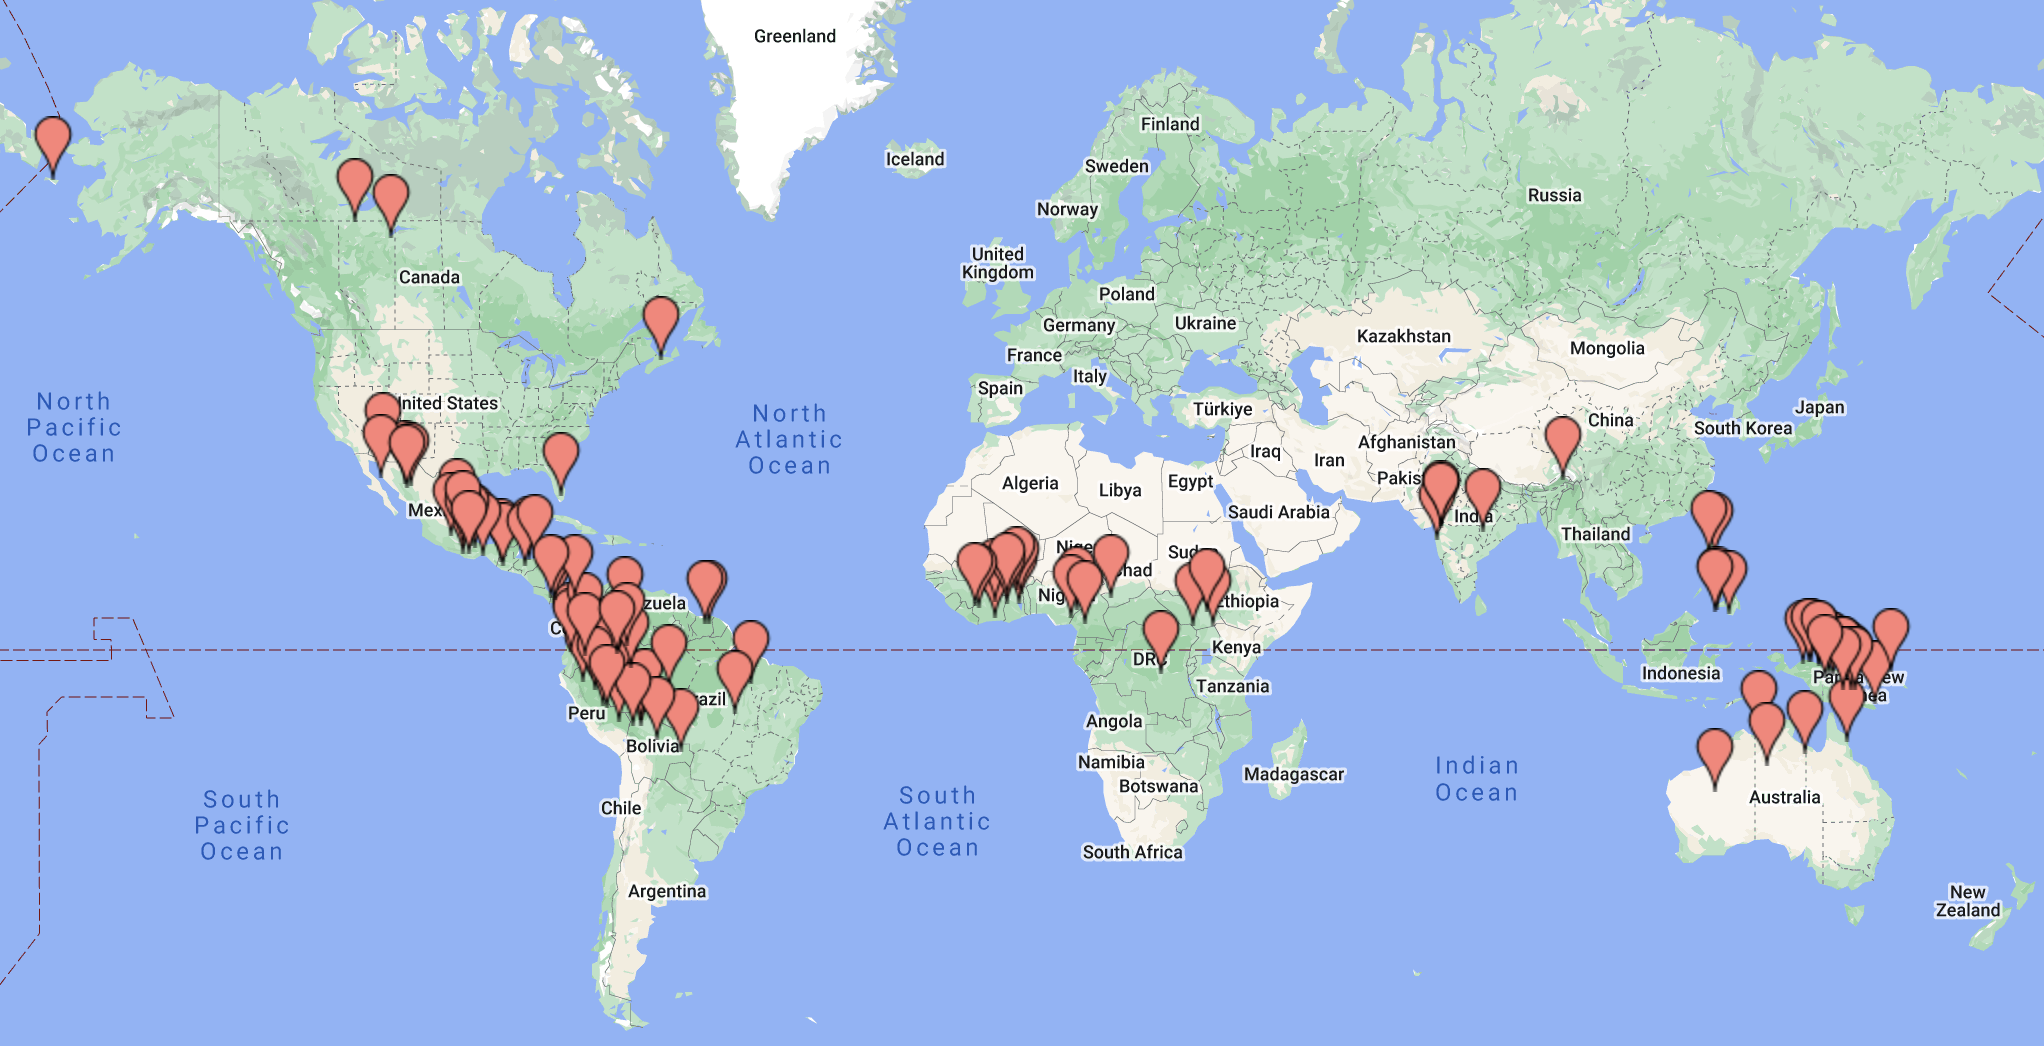
\includegraphics[width=\linewidth]{images/wcs-locations.png}
\decoRule
\caption[WCS Locations]{World map with information on the location of the 110 languages examined in the WCS.}
\label{fig:wcs-locations}
\end{figure}


In the World Color Survey (WCS - 1976 to 1980) data sets of 110 unwritten languages (See locations in Fig. \ref{fig:wcs-locations}) were collected, which were considered to be uncontaminated by contact with highly industrialized cultures 
\parencite{kayWorld2016}.
The procedure was twofold and the collection of Munsell chips was expanded by one white color chip. 
In a first ``free naming task" the participants were presented with each single Munsell chip in a pseudo randomized order and requested to name the respective color using a BCT. From these answers a list of unique BCT were elicited for the second ``focal task". Here participants were asked to name for each unique color term the chip that best represents the color term. This vast data set was then subject to many different analysis approaches.

% Lindsay & Brown (2006) - Universality of color names
\textcite{lindseyUniversality2006} used k-means clustering, taking the naming pattern of each of the WCS participants as input.
This analysis revealed successively forking categories from two to ten.
The step wise results resembled with exceptions very well the actual categories present in the examined WCS languages and English.
In addition, they identified regions of low concordance dividing roughly warm and cold colors across participants in color space.
Both findings indicate consistent tendencies across languages dependent on the number of color terms.

% Regier B&K (2007)Color naming reflects optimal partitions of color space

\begin{figure}[htbp]
\centering
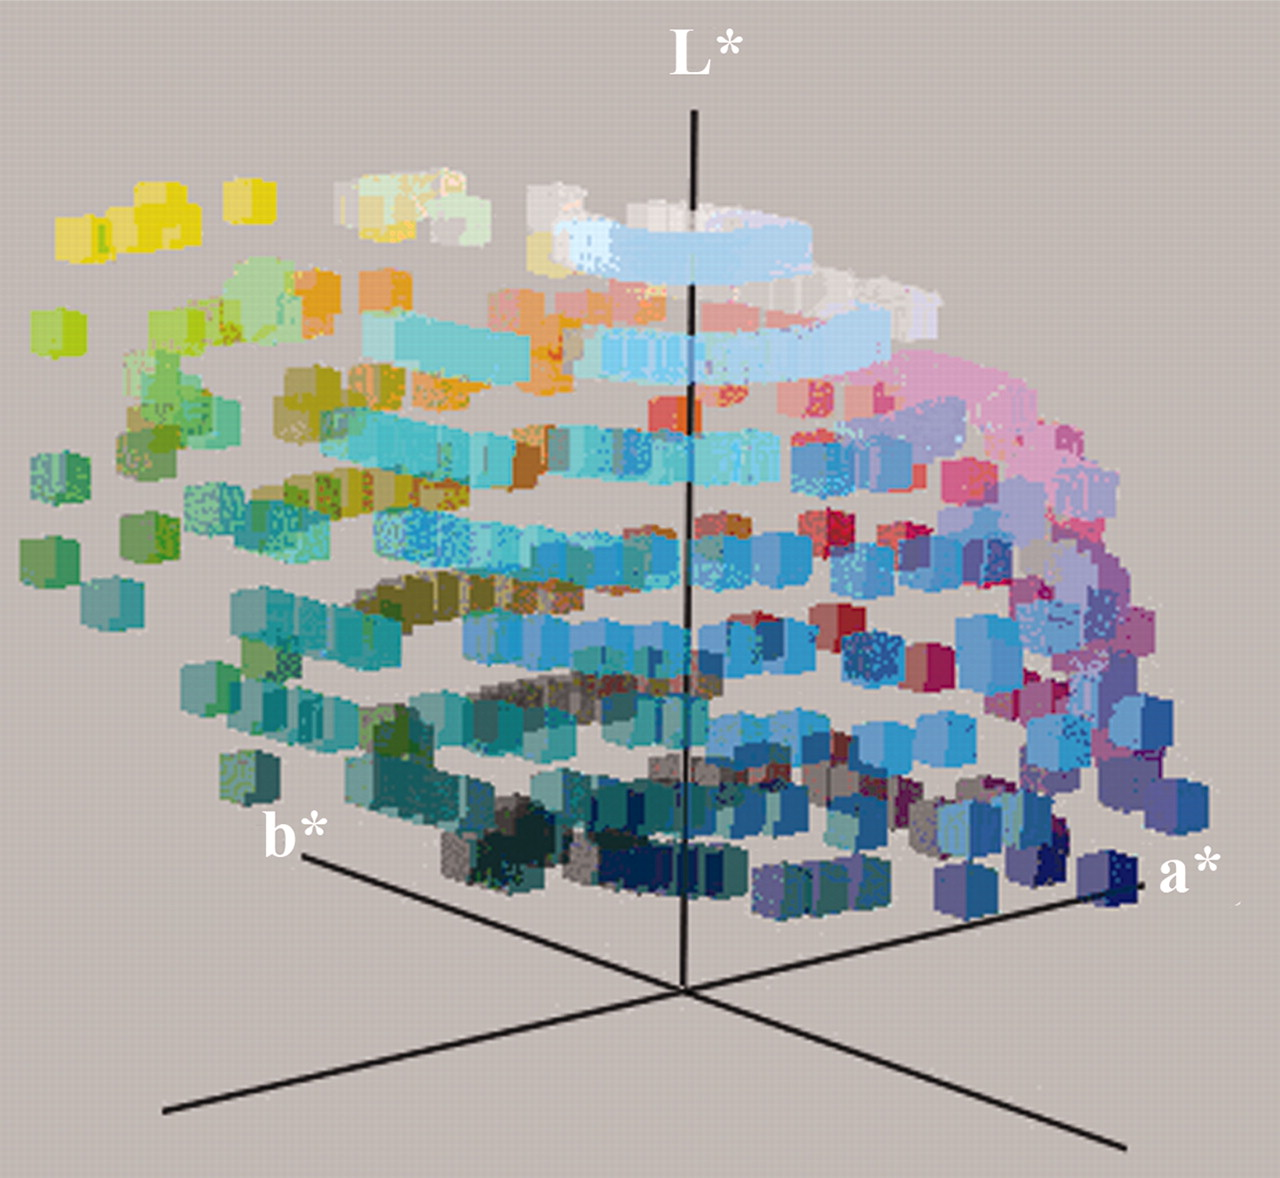
\includegraphics[width=\linewidth]{images/Cielab-space.jpeg}
\decoRule
\caption[Munsell Chips in Cielab Color Space.]{Munsell Chips in Cielab Color Space: 330 Musell color chips projected into Cielab color space. The irregular arrangement of the color chips is most prominent in the yellow region. \textcite{regierColor2007} used this irregularities and principles of categorization to explain the location and shape of color categories.
Taken from \textcite{regierColor2007}.}
\label{fig:Cielab_space}
\end{figure}

Subsequent theoretical work provided an alternative interpretation of the WCS findings. According to \textcite{regierColor2007}, the results of the WCS can be explained from two principles: a) a universally shared visual system, and b) an ``efficient'' organization of the lexicon based on the mere irregularity of color space and basic assumptions of categorization.
When converting the 330 color chips into the CIElab space, which constitutes a better psychophysical representation of color space, the resulting locations of these color values do not yield a perfect symmetric shape (Fig. \ref{fig:Cielab_space}).
A model using euclidean distances between color chips and rules of categorization to minimize similarity across categories and vice versa was able to predict naming patterns of real WCS languages.
A well formedness factor was calculated as the sum of all distances of all chips of the same category and the distances of all chips that do not belong to the same category.
When rotating the naming pattern along the L*axis, meaning to change the region of categories in the CIElab color space, the well formedness factor declined.
This was also true for languages that did not match the optimal model predictions.
Overall, these results support the hypothesis that color categories fit into optimal regions arranged by the universal peculiarities of color space.



% Relativists:
The Sapir-Whorf hypothesis assumes that perception is determined by the categories and filters of language. This approach agrees with the idea that color terminology seeks for optimization but is based on different premises. Color terminology is considered to be shaped by the rules of language rather than by universal properties of the color domain.

% Noga:
% \parenparencite{zaslavskyEfficient2018}
Information Bottleneck (IB) theory posits that language evolution is driven by a dual imperative: a tendency towards simplification for ease of use, while concurrently striving for maximal precision in communication.
\textcite{zaslavskyEfficient2018} showed that the WCS languages achieve nearly optimal communicative efficiency in this trade-off between complexity and information loss.
Following the IB principles, they were able to predict the successive differentiation of the color categories depicted in WCS languages. 
Similarity in naming patterns across languages of equal number of color terms is based on the principle to maximize accuracy given a particular complexity.
The results of an iterated learning experiment performed by \textcite{xuCultural2013} are consistent with this communicative account. In the experiment, English-speaking participants were initially exposed to random assignments of color chips. Participants then generalized their responses to unseen chips after receiving some examples. The result of one participant was given to another participant, imitating cultural transmission in the real world. The systems of color terms produced by this process reproduced the structure of systems of color terms documented in the WCS.


% Color Term Evolution
Regarding Berlin and Kay's evolution hypothesis, followup studies declared to have found additional BCT for Russian \parencite{daviesBasic1994}, Greek \parencite{thierryUnconscious2009}, Turkish \parencite{ozgenTurkish1998} and German\parencite{zollingerWhy1984}.
Specifically, \textcite{winawerRussian2007} found disparities between Russian and English speakers not just in their color nomenclature but also in their ability to quickly and accurately distinguish between colors that belong to separate categories in one language but not the other.
\textcite{kurikiModern2017} have identified a large number of color categories that have evolved in Japanese in less than the last fifty years.
Another study by \textcite{lindseyColor2014} proposed the stabilization of new color terms in English.
Furthermore, they provide evidence for both the emergence \parencite{levinsonYeli2000} and partitioning \parencite{kayLinguistic1978} hypothesis, indicating that new color terms emerge both between existing color categories and through partitioning of old categories.
Across all WCS languages, \textcite{lindsey2009World} were able to categorize individual differences into six motives, reflecting the use of different subsets of BCT. The presence of two motives was replicated for English \parencite{lindseyColor2014}.

% Gibbson:
A large picture corpus investigation by \textcite{gibsonColor2017} addresses the incentives for developing new color terms.
They discovered that objects on pictures are more likely to be colored in warm colors compared to the background.
Secondly, they were able to show that people name warm colors with higher precision and more concise than cold colors.
From this they concluded that the frequency of usage represents an impulse to differentiate between colors and come up with new categories.
In a further part of the study they recruited Tsimane participants. The Tsimane is a group of indigenous farmer-foragers living in remote areas of the Bolivian Amazon basin who are considered to be relatively isolated form western cultural influence \parencite{mcdermott2016indifference}.
When confronted with artificial objects they exhibited a higher usage of diverse color adjectives compared to natural objects.
Thus, industrialization and the crafting of artificial objects using synthetic colors might drive the creation of new color terms.
These results show, that we can not be sure that previous data sets are not outdated by now. Collecting new data could be specifically interesting in terms of deciphering the mechanisms of color term development especially for language exposed to globalization effect.



% \paragraph{\textbf{Color terms}}
\subsection{BCT}
The definition of BCT is non trivial. The study of basic color term has long history and dates back to Homers study about color term usage of the ancient Greek people \parencite{homer2015odyssey} later analysed by \textcite{gladstone1877colour}.
The concept was strongly promoted by aforementioned work by Berlin And Key \parencite{berlinBasic1969}. In this thesis we define BCT to be commonly used in everyday life and not a compound word but a single word. Across the literature different explanations are given and different components are emphasized although this is a key factor to elicit comparable results (\textcite{kayWorld2009},\textcite{lindseyColor2014}). In fact, finding a definition that can be validly generalized across languages is a complex task. Some languages investigated during the WCS did not even have a word for color. In these cases experimenters were asked to use phrases like "How does it strike you eyes" \parencite{kayWorld2016}. In addition, the role and concept of compound words vary strongly across languages and make this definition less explicit. 
%In the case of Vietnamese it is not conclusively evident whether parts of a single word can be seperated by an "-" or if this already indicated that it is a compound word.


Another issue in the literature is the relationship between color terms and color categories. Often these two concepts are used interchangeably or mixed. However, this poses problems, particularly when inferences are made from color terms and their use on color categories. \textcite{lindsey2009World} for example applied a k-means clustering algorithm on each individual naming pattern to identify a reasonable distribution of color categories independent of the actual term assigned. These categories are then named by the most common color term for this category. Even if they justify the level of this threshold the value remains arbitrary and distinct terms might be unified in single color categories. Therefore, in the domain of color terms, clustering terms together is a strong unstable assumption. To avoid this loss of information, in this work we propose an alternative approach that does not commit to one category for each color. 
% Confusion of Color Categories and Terms
% A weakness in the studies mentioned so far is the confusion of color terms and categories.
% For the sake of clustering synonyms into one category the authors used k-means clustering to detect categories.
% However, we understand that in the domain of color terms, clustering terms together is a strong unstable assumption.
% Where to put the threshold to distinguish between two clusters?
% Especially in this research investigating the influence of language on perception we should stick to the actual color terms.
% Therefore, we propose that each color term should be treated as an own category.
% Hence, we strongly depend our analysis on color terms instead of clustered categories.

